\section{Experiments}

We use the crypto data described above to train and test the performance of the different models. Due to computational limitations, we take the last 100k time steps with 90k time steps for training and the last 10k used as a test set. For LSTM and combined models, a sequence of 10 time-steps is taken together as inputs to the model. For GCN, a single frame and the 10-day lookback correlation matrix is used as inputs. Training hyperparameters were tuned manually to find a reasonable best-performing combination.

Our baseline model is a single-layer vanilla LSTM model with a hidden size of 14. Hidden and memory states are initialized to zero tensors. The embeddings at each of the 10 steps is flattened and fed through  Combined models use the baseline model and a single-layer GCN model that uses the above update and creates a 3-dimensional embedding that is then fed through a fully-connected layer to get the point prediction.

\subsection{Results}

\begin{figure}[H]
	\centering
	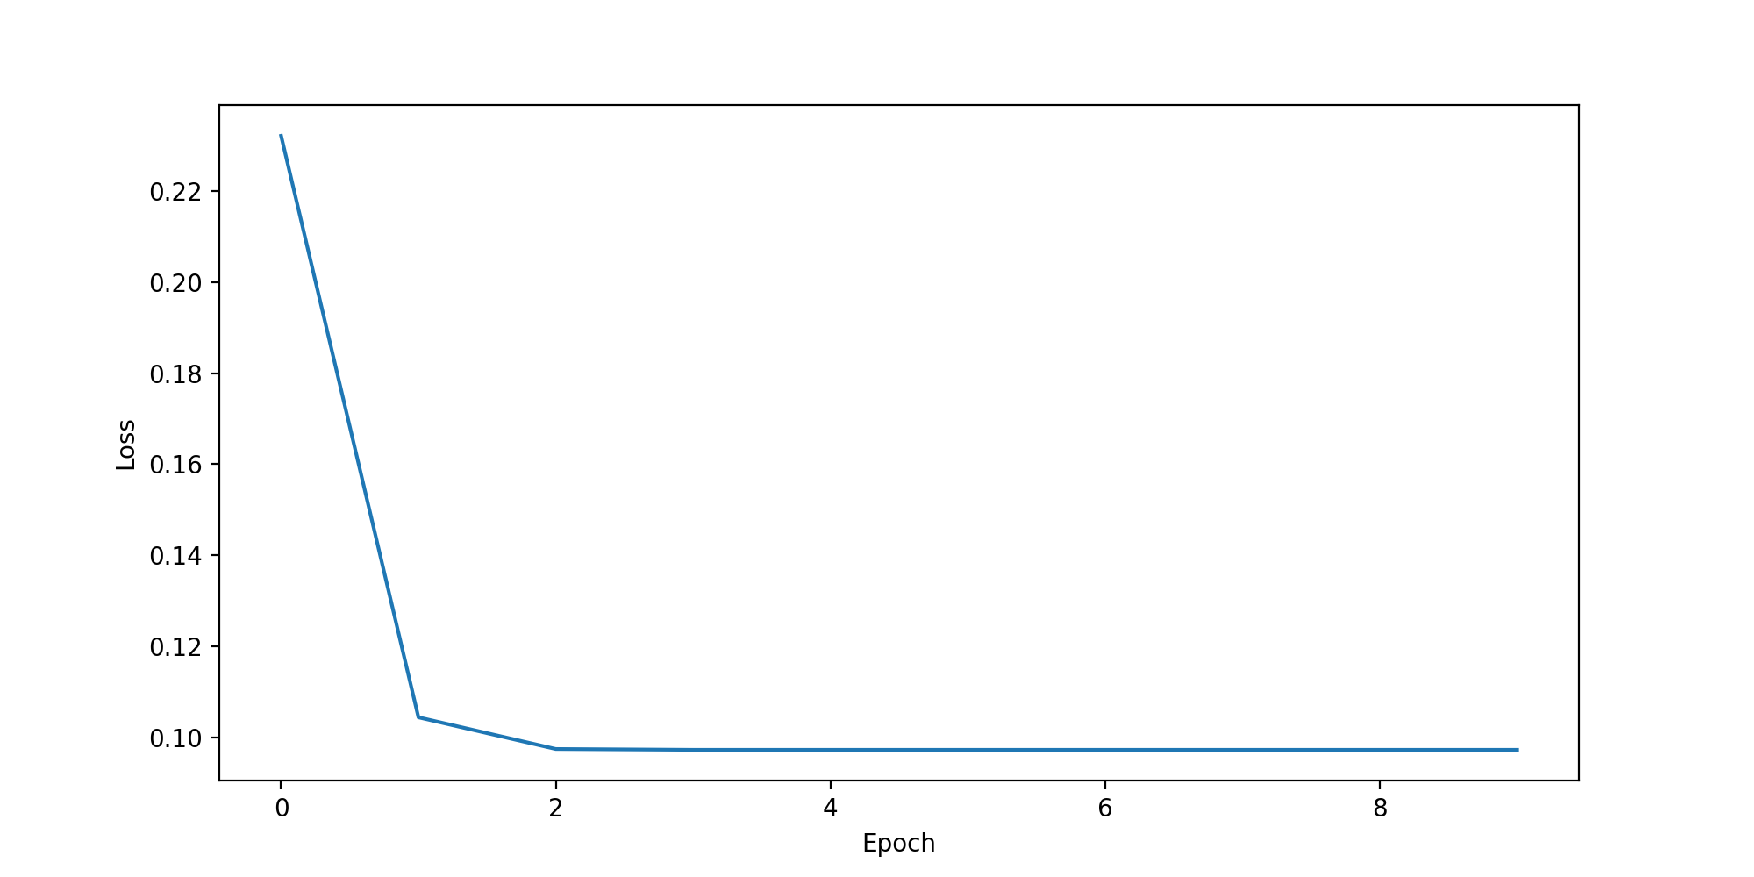
\includegraphics[width=\linewidth]{../../figures/vanilla_lstm_training_loss.pdf}
	\caption{Training loss of baseline LSTM model}
	\label{fig:lstm_loss}
\end{figure}

\begin{table}[H]
	\centering
	\begin{tabular}{|c|c|c|c|c|}
	\hline
	Model & Optimzier & Learning Rate & Momentum & MSE \\
	\hline
	LSTM & SGD & 0.0001 & 0.9 & 0.0030 \\
	Additive & & & & \\
	Sequential & & & & \\
	\hline
	\end{tabular}
	\caption{Hyperparameters for best performing model with average MSE on validation set}
	\label{tab:results_summary}
\end{table}